\documentclass[11pt,reqno]{amsart}

\usepackage[T1]{fontenc}
\usepackage{lmodern}
\usepackage[utf8]{inputenc}
\usepackage{amsmath,amssymb,amsthm,mathtools}
\usepackage{bm}
\usepackage{booktabs}
\usepackage{array}
\usepackage{graphicx}
\usepackage{xcolor}
\usepackage{enumitem}
\usepackage[margin=1.12in]{geometry}
\usepackage{microtype}
\usepackage[hypertexnames=false]{hyperref}
\usepackage{cleveref}

\definecolor{acadblue}{rgb}{0.05,0.22,0.55}
\emergencystretch=1.8em

\hypersetup{
  colorlinks=true,
  linkcolor=acadblue,
  citecolor=acadblue,
  urlcolor=acadblue,
  pdftitle={Heat-Flow PDE Hierarchy on Jensen Invariants, Nodal-Curvature Zero Velocity, and Conditional Saddle Perturbation under De Bruijn-Newman Evolution},
  pdfauthor={Thijs Missiaen}
}

\theoremstyle{plain}
\newtheorem{theorem}{Theorem}[section]
\newtheorem{proposition}[theorem]{Proposition}
\newtheorem{lemma}[theorem]{Lemma}
\newtheorem{corollary}[theorem]{Corollary}

\theoremstyle{definition}
\newtheorem{definition}[theorem]{Definition}

\theoremstyle{remark}
\newtheorem{remark}[theorem]{Remark}

\numberwithin{equation}{section}

\newcommand{\dd}{\,\mathrm{d}}
\newcommand{\ii}{\mathrm{i}}
\newcommand{\ee}{\mathrm{e}}
\newcommand{\fac}{\mathclose{\mathchar"0021}}
\newcommand{\PV}{\mathrm{P.V.}}
\newcommand{\sinch}{\mathrm{sinc}_{\mathrm{hyp}}}
\DeclareMathOperator{\Reop}{Re}
\DeclareMathOperator{\Imop}{Im}

\title[Heat-Flow Jensen PDE Hierarchy and De Bruijn--Newman Evolution]{Heat-Flow PDE Hierarchy on Jensen Invariants, Nodal-Curvature\\ Zero Velocity, and Conditional Saddle Perturbation\\ under De~Bruijn--Newman Evolution}

\author{Thijs Missiaen}
\address{Independent Researcher, Belgium \\ ORCID: \href{https://orcid.org/0009-0007-3678-0810}{0009-0007-3678-0810}}
\email{thijs.missiaen@gmail.com}
\date{October 2026 (Revised Audit Edition)}
\subjclass[2020]{Primary 11M06, 11M26; Secondary 30D15, 35K05}
\keywords{Riemann $\Xi$-function, De~Bruijn--Newman constant, backward heat equation, Jensen invariants, Laguerre--Tur\'an inequalities, nodal curvature, Wigner autocorrelation, Lehmer pairs}

\begin{document}

\begin{abstract}
Let $\Xi_\tau(z) := 8\int_0^\infty \Phi(u)\ee^{\tau u^2}\cos(2zu)\dd u = 8H_\tau(2z)$ be the De~Bruijn--Newman deformation of Riemann's completed zeta function, where $\tau = t_{\mathrm{DBN}}$ is the standard De~Bruijn--Newman parameter ($\partial_\tau\Xi_\tau = -\frac{1}{4}\partial_z^2\Xi_\tau$) and $W_\tau(d,t) := \frac{1}{2}\partial_d\lvert\Xi_\tau(t - \ii d)\rvert^2 = 16\int_0^\infty y\sinh(2dy)I_\tau(y,t)\dd y$. First, we relate the Csordas--Smith--Varga and Rodgers--Tao velocity $\gamma_k'(0) = \Xi''(\gamma_k)/(4\Xi'(\gamma_k))$ to the parabolic curvature $\kappa(\gamma_k)$ of $R(d,t) = 0$ and the extremum curvature on $I(d,t) = 0$. Second, under $y = u + v$, $x = u - v$, we establish the cross-term-free Gaussian Wigner factorization, exhibit the boundary zero $G_{0,\tau}(\ii\eta) = 0$ at $2\eta_0 = 0.63883\dots < \frac{\pi}{4}$, and isolate the numerator condition for pitchfork saddle perturbation. Third, we prove a second-order radial wave-heat PDE for $\widetilde{W}_\tau = W_\tau/d$ and the heat-flow hierarchy $(\partial_\tau + \frac{1}{8}\partial_t^2)L_m(\Xi_\tau; t) = \frac{(m+1)(2m+1)}{4}L_{m+1}(\Xi_\tau; t)$ on all Jensen invariants, yielding the $(m-1)^2/2$ multiple-zero coalescence lift and conditional Lehmer-pair scaling.
\end{abstract}

\maketitle

\section{Introduction}\label{sec:intro}

In the classical theory of the De~Bruijn--Newman constant $\Lambda$ initiated by P\'olya~\cite{polya1926}, de~Bruijn~\cite{debruijn1950}, and Newman~\cite{newman1976}, and developed quantitatively by Csordas, Norfolk, Smith, and Varga~\cite{csordas1986,csordas1988,csordas1994}, Rodgers and Tao~\cite{rodgerstao2020}, and the Polymath~15 collaboration~\cite{polymath2019}, one studies the backward-heat family
\begin{equation}\label{eq:classical_Ht}
H_\tau(x) := \int_0^{\infty} \ee^{\tau u^2}\,\Phi(u)\cos(xu)\dd u, \qquad \Phi(u) := \sum_{n=1}^{\infty} \bigl(2\pi^2 n^4\ee^{9u} - 3\pi n^2\ee^{5u}\bigr)\ee^{-\pi n^2\ee^{4u}},
\end{equation}
satisfying $\partial_\tau H_\tau(x) = -\partial_x^2 H_\tau(x)$, whose zeros are all real if and only if $\tau \ge \Lambda$. The Riemann Hypothesis is equivalent to $\Lambda \le 0$, while Newman's conjecture $\Lambda \ge 0$ was proved unconditionally by Rodgers and Tao~\cite{rodgerstao2020}, and Polymath~15~\cite{polymath2019} established $\Lambda \le 0.22$.

Throughout this series we work in spectral height $z = t - \ii d$ ($s = \frac{1}{2} + d + \ii t$), related to~\eqref{eq:classical_Ht} by $x = 2z$:
\begin{equation}\label{eq:xi_tau_def}
\Xi_\tau(z) := 8\int_0^{\infty} \Phi_\tau(u)\cos(2zu)\dd u = 8\,H_\tau(2z), \qquad \Phi_\tau(u) := \Phi(u)\,\ee^{\tau u^2}.
\end{equation}
Because the Gaussian factor $\ee^{\tau u^2}$ in~\eqref{eq:xi_tau_def} uses the \emph{identical} variable $u$ as~\eqref{eq:classical_Ht}, the heat parameter $\tau$ is identically the standard De~Bruijn--Newman time:
\begin{equation}\label{eq:tau_equals_tdbn}
\tau = t_{\mathrm{DBN}}, \qquad \frac{\partial\Xi_\tau}{\partial\tau}(z) = -\frac{1}{4}\frac{\partial^2\Xi_\tau}{\partial z^2}(z),
\end{equation}
where the prefactor $-\frac{1}{4}$ arises solely from the spatial rescaling $x = 2z$ ($\partial_z^2 = 4\partial_x^2$), and the De~Bruijn--Newman threshold in $\tau$ is $\Lambda$ itself (not $4\Lambda$). At $\tau = 0$, $\Xi_0(z) = \Xi(z) := \xi(\frac{1}{2} + \ii z)$~\cite{riemann1859,titchmarsh1986}. In canonical normalization, the deformed transverse Wronskian and its desingularized quotient $\widetilde{W}_\tau(d,t) := W_\tau(d,t)/d$ read
\begin{equation}\label{eq:canonical_W_tau}
W_\tau(d,t) := \frac{1}{2}\frac{\partial}{\partial d}\bigl\lvert\Xi_\tau(t - \ii d)\bigr\rvert^2 = 16\int_0^{\infty} y\sinh(2dy)\,I_\tau(y,t)\dd y,
\end{equation}
where $I_\tau(y,t) := \int_{-\infty}^{\infty}\Phi_\tau(\frac{y+x}{2})\Phi_\tau(\frac{y-x}{2})\cos(2tx)\dd x$ is the Wigner-type autocorrelation~\cite{wigner1932,hudson1974}. By Speiser~\cite{speiser1934}, de~Branges~\cite{debranges1968}, Hinkkanen~\cite{hinkkanen1997}, and Lagarias~\cite{lagarias1999}, $\Xi_\tau$ is zero-free in $d > 0$ if and only if $W_\tau(d,t) > 0$ on $d > 0$.

\subsection{Proof overview}\label{subsec:overview}

This paper clarifies and proves three connections between the longitudinal evolution~\eqref{eq:tau_equals_tdbn} and the transverse strip geometry $d \ge 0$, separating unconditional differential identities from domain and sign hypotheses:
\begin{enumerate}[label=\textup{(\arabic*)},leftmargin=2.2em]
\item \textbf{Geometric interpretation of the Csordas--Smith--Varga / Rodgers--Tao velocity (\Cref{sec:velocity}).} For simple zeros $x_k(\tau) = 2\gamma_k(\tau)$ of $H_\tau(x)$, Csordas, Smith, and Varga~\cite{csordas1994} and Rodgers and Tao~\cite{rodgerstao2020} proved the Dyson ODE $x_k'(\tau) = H_\tau''(x_k)/H_\tau'(x_k) = 2\,\PV\sum_{j\neq k}(x_k - x_j)^{-1}$, so that $\gamma_k'(0) = \Xi''(\gamma_k)/(4\Xi'(\gamma_k))$ equals $\frac{1}{2}\,\PV\sum_{\gamma_j\neq\gamma_k}(\gamma_k - \gamma_j)^{-1}$. \Cref{prop:nodal_velocity} records the harmonic X-ray interpretation~\cite{speiser1934,ariasdereyna2003}: because $\partial_d^2 R = -\partial_t^2 R$ and $\partial_\tau\Xi_\tau = -\frac{1}{4}\partial_t^2\Xi_\tau$ share the operator $-\partial_t^2$, $\gamma_k'(0) = \frac{1}{4}\kappa(\gamma_k)$ equals one-fourth the parabolic curvature $\kappa(\gamma_k) := t_{\mathcal{R}_k}''(0)$ of $R(d,t) = 0$ at $d = 0$, while critical-line extrema $\tau_k(\tau)$ ($\partial_t\Xi_\tau(\tau_k) = 0$) satisfy $\tau_k'(0) = \frac{3}{4}\kappa_\Gamma(\tau_k)$ relative to $I(d,t)/d = 0$.
\item \textbf{Mirror Gaussian factorization, imaginary-axis kernel zero, and conditional saddle shift (\Cref{sec:wigner}).} Under $y = u + v$, $x = u - v$, the parallelogram identity $u^2 + v^2 = \frac{1}{2}(y^2 + x^2)$ factors $G_{y,\tau}(x) := \Phi_\tau(\frac{y+x}{2})\Phi_\tau(\frac{y-x}{2}) = \ee^{\frac{\tau}{2}y^2}\ee^{\frac{\tau}{2}x^2}G_{y,0}(x)$ without an $xy$ cross-term (\Cref{prop:wigner_factor}). Crucially, however, $G_{y,\tau}(\ii\eta)$ is \emph{not} globally positive on $[0,\infty) \times (-\frac{\pi}{4}, \frac{\pi}{4})$: at $y = 0$, $\Phi(\ii\eta/2)$ vanishes at $2\eta_0 = 0.6388300536\dots < \frac{\pi}{4}$. Restricting to a zero-free neighborhood of a non-degenerate pitchfork saddle $(y_c, \eta_c)$, \Cref{prop:conditional_saddle} derives $\partial_\tau y_c(\omega; 0)$ and $\partial_\tau\eta_c(\omega; 0)$, isolating the numerator inequality $1 - (\partial_y L_{y_c}''(\eta_c))\partial_\tau y_c(\omega; 0) > 0$ required for $\partial_\tau\eta_c(\omega; 0) < 0$.
\item \textbf{Second-order radial wave-heat PDE and the Jensen hierarchy (\Cref{sec:hierarchy}).} Expanding $M_\tau(d,t) := \lvert\Xi_\tau(t - \ii d)\rvert^2 = \sum_{m=0}^\infty L_m(\Xi_\tau; t)\,d^{2m}$ in its classical Jensen--Laguerre Taylor moments~\cite{jensen1913,cravencsordas1989}, \Cref{thm:jensen_pde} proves that $\widetilde{W}_\tau$ obeys a \emph{second-order} radial wave-heat PDE and that every $L_m(f; t)$ of any entire solution to $\partial_\tau f = -\frac{1}{4}\partial_z^2 f$ satisfies the exact ladder identity
\[
\left(\frac{\partial}{\partial\tau} + \frac{1}{8}\frac{\partial^2}{\partial t^2}\right) L_m(f; t) = \frac{(m + 1)(2m + 1)}{4}\,L_{m+1}(f; t) \qquad (m \ge 0),
\]
equivalently $(\partial_\tau + \frac{1}{8}\partial_t^2)c_{2m-1} = \frac{m(2m+1)}{4}c_{2m+1}$ for $c_{2m-1} = m\,L_m$ ($m \ge 1$). \Cref{cor:coalescence_lehmer} deduces the exact multiple-zero lift $\partial_\tau c_{2m-3}(t_0;\tau_{\mathrm{coal}}) = \frac{(m-1)^2}{2}c_{2m-1}(t_0;\tau_{\mathrm{coal}}) > 0$ for all $m \ge 2$ (verified symbolically on heat polynomials $P_m(t,\tau) = \ee^{-\frac{\tau}{4}\partial_t^2}t^m$) and formulates the conditional midpoint inequality governing close Lehmer pairs in $\tau = t_{\mathrm{DBN}}$ within the Csordas--Norfolk--Varga~\cite{csordas1988} lower-bound regime.
\end{enumerate}

\subsection{Notation and conventions}\label{subsec:notation}

Throughout, $s = \sigma + \ii t$ with $d := \sigma - \frac{1}{2} \in \mathbb{R}$, $z := t - \ii d \in \mathbb{C}$, and $\tau = t_{\mathrm{DBN}} \in \mathbb{R}$. We decompose $\Xi_\tau(t - \ii d) = R_\tau(d,t) + \ii I_\tau(d,t)$ with $R_\tau, I_\tau \in \mathbb{R}$ for $(d,t,\tau) \in \mathbb{R}^3$. At $\tau = 0$, the positive real zeros of $\Xi(t)$ are $0 < \gamma_1 < \gamma_2 < \dots$, with symmetric Hadamard roots $\gamma_{-m} := -\gamma_m$. We set $\sinch(w) := \sinh(w)/w$ for $w \neq 0$ and $\sinch(0) := 1$. For any real entire function $f$, the $m$-th Jensen--Laguerre invariant~\cite{jensen1913,cravencsordas1989} is the $d^{2m}$-Taylor coefficient of $\lvert f(t - \ii d)\rvert^2 = f(t - \ii d)f(t + \ii d)$:
\begin{equation}\label{eq:Lm_def}
L_m(f; t) := \sum_{j=0}^{2m} \frac{(-1)^{j+m}}{j\fac\,(2m - j)\fac}\,f^{(j)}(t)\,f^{(2m-j)}(t) \qquad (m \ge 0),
\end{equation}
so that $\widetilde{W}_\tau(d,t) := \frac{1}{2d}\partial_d\lvert\Xi_\tau(t - \ii d)\rvert^2 = \sum_{m=1}^{\infty} c_{2m-1}(t;\tau)\,d^{2m-2}$ has coefficients $c_{2m-1}(t;\tau) = m\,L_m(\Xi_\tau; t)$ ($m \ge 1$). Note that the index upper limit in~\eqref{eq:Lm_def} is $2m$ (an odd upper limit $2m - 1$ would vanish identically by antisymmetry $j \leftrightarrow 2m - 1 - j$).

\section{Nodal-Curvature Interpretation of the Csordas--Smith--Varga Velocity}\label{sec:velocity}

We first record the exact relation between the classical De~Bruijn--Newman zero-velocity formula~\cite{csordas1994,rodgerstao2020,polymath2019} and the critical-line nodal curvatures of $\Xi(t - \ii d) = R(d,t) + \ii I(d,t)$~\cite{speiser1934,ariasdereyna2003}.

\begin{proposition}[Nodal-curvature interpretation of initial zero and extremum velocities]\label{prop:nodal_velocity}
For all $(z,\tau) \in \mathbb{C} \times \mathbb{R}$, $\Xi_\tau(z)$ in~\eqref{eq:xi_tau_def} is an even entire function of order one satisfying $\partial_\tau\Xi_\tau(z) = -\frac{1}{4}\partial_z^2\Xi_\tau(z)$ with $\tau = t_{\mathrm{DBN}}$.
\begin{enumerate}[label=\textup{(\roman*)},leftmargin=2.2em]
\item \textbf{Simple zeros and real nodal curvature.} Let $\gamma_k$ be a simple real zero of $\Xi(t)$ ($\Xi(\gamma_k) = 0$, $\Xi'(\gamma_k) \neq 0$). By the implicit function theorem, there exist unique real-analytic branches $\gamma_k(\tau)$ solving $\Xi_\tau(\gamma_k(\tau)) = 0$ near $\tau = 0$ and $t_{\mathcal{R}_k}(d)$ solving $R(d, t_{\mathcal{R}_k}(d)) = 0$ near $d = 0$, with $t_{\mathcal{R}_k}(0) = \gamma_k$, $t_{\mathcal{R}_k}'(0) = 0$, and parabolic curvature $\kappa(\gamma_k) := t_{\mathcal{R}_k}''(0) = \Xi''(\gamma_k)/\Xi'(\gamma_k)$. The Csordas--Smith--Varga / Rodgers--Tao velocity at $\tau = 0$ satisfies
\begin{equation}\label{eq:zero_velocity_curvature}
\gamma_k'(0) = \frac{\Xi''(\gamma_k)}{4\,\Xi'(\gamma_k)} = \frac{1}{4}\,\kappa(\gamma_k) = \frac{1}{2}\,\PV\sum_{\gamma_j \neq \gamma_k} \frac{1}{\gamma_k - \gamma_j},
\end{equation}
where $\PV\sum_{\gamma_j \neq \gamma_k}(\gamma_k - \gamma_j)^{-1} := \frac{1}{2\gamma_k} + \sum_{m \ge 1,\, m \neq k} \frac{2\gamma_k}{\gamma_k^2 - \gamma_m^2}$ sums symmetrically over $\pm\gamma_m$.
\item \textbf{Critical-line extrema and imaginary nodal curvature.} Let $\tau_k$ be a non-degenerate critical-line extremum of $\Xi(t)$ ($\Xi'(\tau_k) = 0$, $\Xi''(\tau_k) \neq 0$). Near $\tau = 0$ and $d = 0$, the extremum locus $\partial_t\Xi_\tau(\tau_k(\tau)) = 0$ and the desingularized imaginary nodal curve $I(d, \tau_{\Gamma_k}(d))/d = 0$ ($\tau_{\Gamma_k}(0) = \tau_k$, $\tau_{\Gamma_k}'(0) = 0$) satisfy
\begin{equation}\label{eq:extremum_velocity_curvature}
\tau_k'(0) = \frac{\Xi'''(\tau_k)}{4\,\Xi''(\tau_k)} = \frac{3}{4}\,\kappa_\Gamma(\tau_k), \qquad \kappa_\Gamma(\tau_k) := \tau_{\Gamma_k}''(0) = \frac{\Xi'''(\tau_k)}{3\,\Xi''(\tau_k)}.
\end{equation}
\end{enumerate}
\end{proposition}

\begin{proof}
Since $\lvert\Phi(u)\rvert \ll \ee^{9\lvert u\rvert}\exp(-\pi\ee^{4\lvert u\rvert})$, $\Phi(u)\ee^{\tau u^2}(2u)^{2k}\cos(2zu)$ is majorized uniformly on compact subsets of $\mathbb{C} \times \mathbb{R}$ by an integrable function, so differentiating~\eqref{eq:xi_tau_def} under the integral sign brings down $u^2$ for $\partial_\tau$ and $-4u^2$ for $\partial_z^2$, giving $\partial_\tau\Xi_\tau = -\frac{1}{4}\partial_z^2\Xi_\tau$.

For~(i), implicit differentiation of $\Xi_\tau(\gamma_k(\tau)) = 0$ at $\tau = 0$ gives $\partial_\tau\Xi_0(\gamma_k) + \Xi'(\gamma_k)\gamma_k'(0) = 0$, hence $\gamma_k'(0) = \Xi''(\gamma_k)/(4\Xi'(\gamma_k))$~\cite{csordas1994,rodgerstao2020}. Expanding $\Xi(\gamma_k + \Delta t - \ii d) = \Xi'(\gamma_k)(\Delta t - \ii d) + \frac{1}{2}\Xi''(\gamma_k)(\Delta t - \ii d)^2 + \mathcal{O}((\lvert\Delta t\rvert + \lvert d\rvert)^3)$ and taking real parts yields $R(d, \gamma_k + \Delta t) = \Xi'(\gamma_k)\Delta t + \frac{1}{2}\Xi''(\gamma_k)(\Delta t^2 - d^2) + \mathcal{O}(d^3) = 0$, so $t_{\mathcal{R}_k}(d) = \gamma_k + \frac{\Xi''(\gamma_k)}{2\Xi'(\gamma_k)}d^2 + \mathcal{O}(d^4)$ and $\kappa(\gamma_k) = t_{\mathcal{R}_k}''(0) = \Xi''(\gamma_k)/\Xi'(\gamma_k)$. Finally, from Hadamard's product $\Xi(z) = \Xi(0)\prod_{m=1}^\infty(1 - z^2/\gamma_m^2)$, writing $\Xi(z) = (z - \gamma_k)g_k(z)$ gives $\Xi''(\gamma_k)/\Xi'(\gamma_k) = 2g_k'(\gamma_k)/g_k(\gamma_k) = \frac{1}{\gamma_k} + \sum_{m \neq k}\frac{4\gamma_k}{\gamma_k^2 - \gamma_m^2}$~\cite{csordas1994}, yielding~\eqref{eq:zero_velocity_curvature}.

For~(ii), differentiating $\partial_t\Xi_\tau(\tau_k(\tau)) = 0$ with $\partial_\tau\partial_t\Xi_0 = -\frac{1}{4}\Xi'''$ gives $\tau_k'(0) = \Xi'''(\tau_k)/(4\Xi''(\tau_k))$. Expanding $\Xi(\tau_k + \Delta t - \ii d)$ with $\Xi'(\tau_k) = 0$ and taking imaginary parts gives
\[
\frac{I(d, \tau_k + \Delta t)}{-d} = \Xi''(\tau_k)\Delta t - \frac{1}{6}\Xi'''(\tau_k)(d^2 - 3\Delta t^2) + \mathcal{O}(d^3) = 0,
\]
whence $\tau_{\Gamma_k}(d) = \tau_k + \frac{\Xi'''(\tau_k)}{6\Xi''(\tau_k)}d^2 + \mathcal{O}(d^4)$ and $\kappa_\Gamma(\tau_k) = \tau_{\Gamma_k}''(0) = \Xi'''(\tau_k)/(3\Xi''(\tau_k))$.
\end{proof}

\begin{table}[htbp]
\centering
\caption{Nodal curvatures $\kappa(\gamma_k) = t_{\mathcal{R}_k}''(0)$, initial zero velocities $\gamma_k'(0) = \frac{1}{4}\kappa(\gamma_k)$ ($\tau = t_{\mathrm{DBN}}$), central finite-difference residuals ($\varepsilon_\tau = 10^{-10}$), and Riemann--von Mangoldt tail-corrected Dyson residuals ($N = 400$ pairs) for the first eight nontrivial zeros.}\label{tab:velocities}
\small
\begin{tabular}{@{}rccccc@{}}
\toprule
$k$ & $\gamma_k$ & $\kappa(\gamma_k) = \Xi''/\Xi'$ & $\gamma_k'(0)$ ($\tau = t_{\mathrm{DBN}}$) & $\lvert\gamma_k'(0) - \mathrm{FD}\rvert$ & $\lvert\gamma_k'(0) - \mathrm{Dyson}_{400}\rvert$ \\
\midrule
$1$ & $14.13472514$ & $-1.1592612$ & $-0.2898153$ & $9.97 \times 10^{-26}$ & $2.84 \times 10^{-6}$ \\
$2$ & $21.02203964$ & $-1.5099908$ & $-0.3774977$ & $9.21 \times 10^{-25}$ & $4.23 \times 10^{-6}$ \\
$3$ & $25.01085758$ & $-1.1716664$ & $-0.2929166$ & $1.35 \times 10^{-24}$ & $5.04 \times 10^{-6}$ \\
$4$ & $30.42487613$ & $-1.9108425$ & $-0.4777106$ & $1.61 \times 10^{-23}$ & $6.13 \times 10^{-6}$ \\
$5$ & $32.93506159$ & $-0.9308909$ & $-0.2327227$ & $1.66 \times 10^{-23}$ & $6.64 \times 10^{-6}$ \\
$6$ & $37.58617816$ & $-1.6773339$ & $-0.4193335$ & $1.21 \times 10^{-24}$ & $7.58 \times 10^{-6}$ \\
$7$ & $40.91871901$ & $-1.7149223$ & $-0.4287306$ & $1.54 \times 10^{-23}$ & $8.26 \times 10^{-6}$ \\
$8$ & $43.32707328$ & $-0.8986902$ & $-0.2246726$ & $1.76 \times 10^{-23}$ & $8.75 \times 10^{-6}$ \\
\bottomrule
\end{tabular}
\end{table}

\section{Mirror Gaussian Factorization, Boundary Root $2\eta_0$, and Conditional Saddle Shift}\label{sec:wigner}

Substituting $\Xi_\tau(t - \ii d) = 4\int_{-\infty}^\infty \Phi_\tau(u)\ee^{2du}\ee^{-2\ii tu}\dd u$ into~\eqref{eq:canonical_W_tau} and changing variables to mirror coordinates $y = u + v$, $x = u - v$ ($\dd u\dd v = \frac{1}{2}\dd x\dd y$) yields the canonical integral representation~\eqref{eq:canonical_W_tau}:
\begin{equation}\label{eq:W_tau_canonical_full}
W_\tau(d,t) = 16\int_0^{\infty} y\sinh(2dy)\,I_\tau(y,t)\dd y, \qquad \widetilde{W}_\tau(d,t) = 32\int_0^{\infty} y^2\sinch(2dy)\,I_\tau(y,t)\dd y,
\end{equation}
where $I_\tau(y,t) = \int_{-\infty}^{\infty} G_{y,\tau}(x)\cos(\omega x)\dd x$ with $\omega := 2t$ and $G_{y,\tau}(x) := \Phi_\tau(\frac{y+x}{2})\Phi_\tau(\frac{y-x}{2})$.

\begin{proposition}[Mirror Gaussian factorization and boundary zero at $2\eta_0 < \frac{\pi}{4}$]\label{prop:wigner_factor}
For all $(y,x,\tau) \in [0,\infty) \times \mathbb{C} \times \mathbb{R}$, the identity $\bigl(\frac{y+x}{2}\bigr)^2 + \bigl(\frac{y-x}{2}\bigr)^2 = \frac{1}{2}(y^2 + x^2)$ yields the cross-term-free factorization and Wigner PDE
\begin{equation}\label{eq:mirror_factor}
G_{y,\tau}(x) = \ee^{\frac{\tau}{2}y^2}\,\ee^{\frac{\tau}{2}x^2}\,G_{y,0}(x), \qquad \frac{\partial I_\tau}{\partial\tau}(y,t) = \frac{1}{8}\left(4y^2 - \frac{\partial^2}{\partial t^2}\right)I_\tau(y,t),
\end{equation}
and $G_{y,\tau}(x)$ remains entire in $x$ with rapid horizontal decay on every strip $\lvert\Imop(x)\rvert \le \frac{\pi}{4} - \varepsilon$ ($\varepsilon > 0$). However, $G_{y,\tau}(\ii\eta)$ is \emph{not} everywhere strictly positive on $[0,\infty) \times (-\frac{\pi}{4}, \frac{\pi}{4})$: along the boundary slice $y = 0$, $G_{0,\tau}(\ii\eta) = \ee^{-\frac{\tau}{2}\eta^2}\lvert\Phi(\ii\eta/2)\rvert^2$ vanishes inside $(0, \frac{\pi}{4})$ at
\begin{equation}\label{eq:two_eta0_root}
\eta_* := 2\eta_0 = 0.63883005360059357748\dots < \frac{\pi}{4} = 0.78539816339744830962\dots,
\end{equation}
where $\Phi(\ii\eta_0) = 0$, creating a logarithmic singularity in $\ln G_{0,\tau}(\ii\eta)$ at $\eta = \pm 2\eta_0$.
\end{proposition}

\begin{proof}
Since $\Phi_\tau(u) = \Phi(u)\ee^{\tau u^2}$, $G_{y,\tau}(x) = \ee^{\tau((\frac{y+x}{2})^2 + (\frac{y-x}{2})^2)}G_{y,0}(x) = \ee^{\frac{\tau}{2}(y^2+x^2)}G_{y,0}(x)$. Differentiating $I_\tau(y,t) = \int_{-\infty}^\infty \ee^{\frac{\tau}{2}(y^2+x^2)}G_{y,0}(x)\cos(2tx)\dd x$ under the integral sign brings down $\frac{1}{2}(y^2 + x^2)$, while $\partial_t^2\cos(2tx) = -4x^2\cos(2tx)$, proving~\eqref{eq:mirror_factor}. On $x = \xi + \ii\eta$ with $\lvert\eta\rvert \le \frac{\pi}{4} - \varepsilon$, $\Reop(\ee^{2(y\pm x)}) = \ee^{2(y\pm\xi)}\cos(2\eta) \ge \sin(2\varepsilon)\ee^{2(y\pm\xi)}$, so the double-exponential factor $\exp(-\pi\sin(2\varepsilon)(\ee^{2(y+\xi)} + \ee^{2(y-\xi)}))$ dominates $\ee^{\frac{\tau}{2}(\xi^2 - \eta^2)}$ as $\lvert\xi\rvert \to \infty$ for every $\tau \in \mathbb{R}$. Finally, at $y = 0$ and $x = \ii\eta$, $G_{0,\tau}(\ii\eta) = \ee^{-\frac{\tau}{2}\eta^2}\Phi(\ii\eta/2)\Phi(-\ii\eta/2) = \ee^{-\frac{\tau}{2}\eta^2}\lvert\Phi(\ii\eta/2)\rvert^2$. Since $\Phi(\ii\cdot 0.30) = +2.9656\dots > 0$ and $\Phi(\ii\cdot 0.35) = -13.8666\dots < 0$, $\Phi(\ii u)$ has a real root $\eta_0 = 0.31941502680029678874\dots \in (0, \frac{\pi}{8})$, so $G_{0,\tau}(\ii\eta)$ vanishes at $\eta_* = 2\eta_0 < \frac{\pi}{4}$.
\end{proof}

Because of~\eqref{eq:two_eta0_root}, logarithmic saddle-point equations require restricting to open zero-free subdomains $\mathcal{U} \subset (0,\infty) \times (0, \frac{\pi}{4})$ on which $\Phi(\frac{y + \ii\eta}{2}) \neq 0$, and the sign of $\partial_\tau\eta_c$ depends on an explicit two-term numerator condition rather than following from $\partial_\tau y_c > 0$ alone.

\begin{proposition}[Conditional perturbation of a local pitchfork saddle]\label{prop:conditional_saddle}
Let $\omega = 2t > 0$, and suppose $(y_c(\omega; 0), \eta_c(\omega; 0)) \in (0,\infty) \times (0, \frac{\pi}{4})$ lies in a zero-free neighborhood $\mathcal{U}$ where $\Phi(\frac{y + \ii\eta}{2}) \neq 0$, so that $L_{y,\tau}(\eta) := \ln G_{y,\tau}(\ii\eta) = L_y(\eta) + \frac{\tau}{2}(y^2 - \eta^2)$ with $L_y(\eta) := 2\ln\lvert\Phi(\frac{y + \ii\eta}{2})\rvert$ is real-analytic on $\mathcal{U}$. Assume $(y_c(\omega; 0), \eta_c(\omega; 0))$ solves the $\tau = 0$ pitchfork saddle-coalescence system $L_{y_c}'(\eta_c) = \omega$, $L_{y_c}''(\eta_c) = 0$ with non-zero Jacobian determinant $\Delta_J := -(\partial_y L_{y_c}'(\eta_c))\,L_{y_c}'''(\eta_c) \neq 0$. Then for $\lvert\tau\rvert$ sufficiently small there exists a unique real-analytic branch $(y_c(\omega;\tau), \eta_c(\omega;\tau))$ solving $L_{y_c}'(\eta_c) - \tau\eta_c = \omega$ and $L_{y_c}''(\eta_c) = \tau$, with initial derivatives at $\tau = 0$:
\begin{equation}\label{eq:saddle_velocities}
\left.\frac{\partial y_c(\omega;\tau)}{\partial\tau}\right|_{\tau=0} = \frac{\eta_c(\omega; 0)}{\partial_y L_{y_c}'\bigl(\eta_c(\omega; 0)\bigr)}, \qquad \left.\frac{\partial\eta_c(\omega;\tau)}{\partial\tau}\right|_{\tau=0} = \frac{1 - \bigl(\partial_y L_{y_c}''(\eta_c)\bigr)\,\partial_\tau y_c(\omega; 0)}{L_{y_c}'''\bigl(\eta_c(\omega; 0)\bigr)}.
\end{equation}
In particular, if $\partial_y L_{y_c}'(\eta_c) > 0$ and $L_{y_c}'''(\eta_c) < 0$, then $\partial_\tau y_c(\omega; 0) > 0$ holds unconditionally, whereas $\partial_\tau\eta_c(\omega; 0) < 0$ holds \emph{if and only if} the numerator condition
\begin{equation}\label{eq:numerator_condition}
1 - \bigl(\partial_y L_{y_c}''(\eta_c)\bigr)\,\partial_\tau y_c(\omega; 0) > 0
\end{equation}
is satisfied at $(y_c(\omega; 0), \eta_c(\omega; 0))$.
\end{proposition}

\begin{proof}
On $\mathcal{U}$, $\partial_\eta[L_{y,\tau}(\eta) - \omega\eta] = L_y'(\eta) - \tau\eta - \omega$ and $\partial_\eta^2[L_{y,\tau}(\eta) - \omega\eta] = L_y''(\eta) - \tau$. At $\tau = 0$, the Jacobian matrix with respect to $(y,\eta)$ at $L_{y_c}''(\eta_c) = 0$ is $\bigl(\begin{smallmatrix} \partial_y L_{y_c}' & 0 \\ \partial_y L_{y_c}'' & L_{y_c}''' \end{smallmatrix}\bigr)$, whose determinant $\Delta_J = (\partial_y L_{y_c}')L_{y_c}'''$ is non-zero by hypothesis. Differentiating $L_{y_c}'(\eta_c) - \tau\eta_c = \omega$ at $\tau = 0$ gives $(\partial_y L_{y_c}')\partial_\tau y_c + L_{y_c}''\partial_\tau\eta_c - \eta_c = 0$; since $L_{y_c}''(\eta_c) = 0$, the first formula in~\eqref{eq:saddle_velocities} follows. Differentiating $L_{y_c}''(\eta_c) - \tau = 0$ at $\tau = 0$ gives $(\partial_y L_{y_c}'')\partial_\tau y_c + L_{y_c}'''\partial_\tau\eta_c - 1 = 0$, giving the second formula in~\eqref{eq:saddle_velocities}. When $L_{y_c}'''(\eta_c) < 0$, the quotient has negative sign if and only if its numerator~\eqref{eq:numerator_condition} is strictly positive.
\end{proof}

At $\omega_1 = 2\gamma_1 = 28.26945028\dots$, $50$-digit root-finding gives $y_c = 0.43202053\dots$ and $\eta_c = 0.60271502\dots$, where $\lvert\Phi(\frac{y_c+\ii\eta_c}{2})\rvert = 9.07589\dots > 0$, $\partial_\tau y_c(2\gamma_1; 0) = +0.01253623\dots > 0$, and the numerator~\eqref{eq:numerator_condition} equals $+0.40397876\dots > 0$, yielding $\partial_\tau\eta_c(2\gamma_1; 0) = -3.760863\dots \times 10^{-4} < 0$. Proving~\eqref{eq:numerator_condition} uniformly for all $\omega \to \infty$ remains open.

\begin{figure}[htbp]
\centering
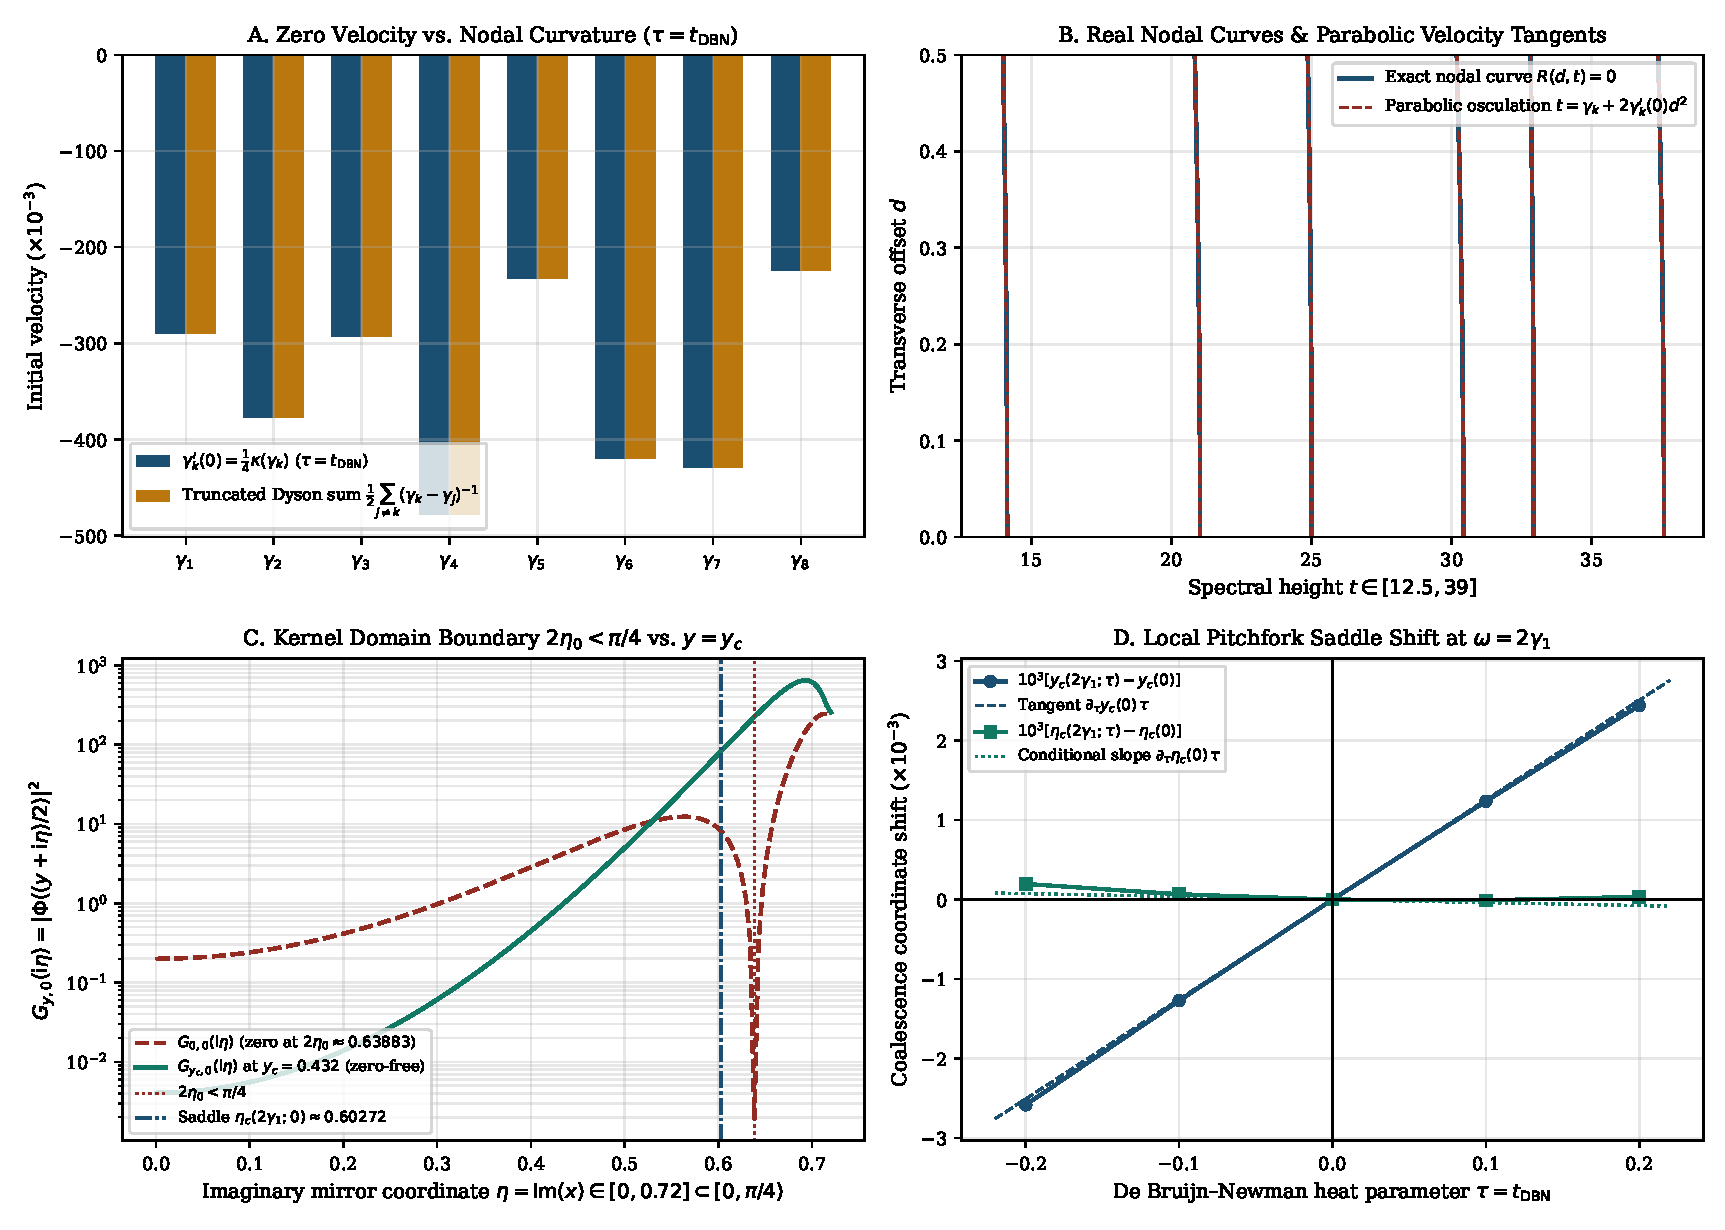
\includegraphics[width=0.97\textwidth]{figures/fig1_debruijn_newman_chladni_velocity_and_wigner.pdf}
\caption{\textbf{A.} Initial zero velocities $\gamma_k'(0) = \frac{1}{4}\kappa(\gamma_k)$ ($\tau = t_{\mathrm{DBN}}$) versus the tail-corrected Dyson sum for $k = 1, \dots, 8$. \textbf{B.} Exact real nodal curves $R(d,t) = 0$ and parabolic osculations $t = \gamma_k + 2\gamma_k'(0)d^2$. \textbf{C.} Boundary root $G_{0,0}(\ii\eta) = 0$ at $2\eta_0 \approx 0.63883 < \frac{\pi}{4}$ versus the zero-free slice $y = y_c(2\gamma_1; 0) \approx 0.432$. \textbf{D.} Local pitchfork saddle trajectories $(y_c(\tau), \eta_c(\tau))$ at $\omega = 2\gamma_1$.}\label{fig:fig1}
\end{figure}

\section{Second-Order Radial Wave-Heat PDE and the Heat-Flow Hierarchy on Jensen Invariants}\label{sec:hierarchy}

We now prove the central exact differential hierarchy of this paper, governing the evolution of $\widetilde{W}_\tau(d,t)$ and of all Jensen--Laguerre Taylor invariants $L_m(\Xi_\tau; t)$ and $c_{2m-1}(t;\tau) = m\,L_m(\Xi_\tau; t)$ under the backward heat flow. Note that the radial PDE for $\widetilde{W}_\tau$ is of \emph{second order} in $(d,t)$ (whereas $\widetilde{W}_{1,2;\tau}$ involves third-order derivatives of $\Xi_\tau$).

\begin{theorem}[Second-order radial wave-heat PDE and heat-flow PDE hierarchy on Jensen invariants]\label{thm:jensen_pde}
Let $f(z,\tau)$ be any real-analytic entire family on $\mathbb{C} \times \mathbb{R}$ satisfying $\partial_\tau f = -\frac{1}{4}\partial_z^2 f$ and $\overline{f(z,\tau)} = f(\bar{z},\tau)$, and set $M(d,t;\tau) := \lvert f(t - \ii d,\tau)\rvert^2 = \sum_{m=0}^\infty L_m(f; t)\,d^{2m}$ and $\widetilde{W}_f(d,t;\tau) := \frac{1}{2d}\partial_d M(d,t;\tau) = \sum_{m=1}^\infty c_{2m-1}(t;\tau)\,d^{2m-2}$ with $c_{2m-1} = m\,L_m$.
\begin{enumerate}[label=\textup{(\roman*)},leftmargin=2.2em]
\item \textbf{Second-order wave-heat and radial PDEs.} For all $(d,t,\tau) \in \mathbb{R}^3$, $M$ and $\widetilde{W}_f$ satisfy the exact second-order partial differential equations
\begin{equation}\label{eq:wave_heat_M_W}
\left(\frac{\partial}{\partial\tau} + \frac{1}{8}\frac{\partial^2}{\partial t^2}\right) M = \frac{1}{8}\frac{\partial^2 M}{\partial d^2}, \qquad \frac{\partial\widetilde{W}_f}{\partial\tau} + \frac{1}{8}\left(\frac{\partial^2\widetilde{W}_f}{\partial t^2} - \frac{\partial^2\widetilde{W}_f}{\partial d^2} - \frac{2}{d}\frac{\partial\widetilde{W}_f}{\partial d}\right) = 0,
\end{equation}
together with $\partial_\tau\widetilde{W}_f + \frac{1}{4}\partial_t^2\widetilde{W}_f = \frac{1}{2}\widetilde{W}_{f'}(d,t;\tau)$, where $\widetilde{W}_{f'} := \frac{1}{2d}\partial_d\lvert f'(t - \ii d,\tau)\rvert^2$.
\item \textbf{Exact heat-flow PDE hierarchy on Jensen invariants.} Every Jensen--Laguerre invariant $L_m(f; t)$ ($m \ge 0$) and every Wronskian Taylor coefficient $c_{2m-1}(t;\tau) = m\,L_m(f; t)$ ($m \ge 1$) satisfies
\begin{equation}\label{eq:boxed_jensen_pde}
\boxed{\;\begin{aligned}
\left(\frac{\partial}{\partial\tau} + \frac{1}{8}\frac{\partial^2}{\partial t^2}\right) L_m(f; t) &= \frac{(m + 1)(2m + 1)}{4}\,L_{m+1}(f; t) \qquad (m \ge 0), \\
\left(\frac{\partial}{\partial\tau} + \frac{1}{8}\frac{\partial^2}{\partial t^2}\right) c_{2m-1}(t;\tau) &= \frac{m(2m + 1)}{4}\,c_{2m+1}(t;\tau) \qquad (m \ge 1).
\end{aligned}\;}
\end{equation}
For $f = \Xi_\tau$, each Wronskian moment also admits the canonical integral representation
\begin{equation}\label{eq:cm_integral}
c_{2m-1}(t;\tau) = m\,L_m(\Xi_\tau; t) = \frac{8}{(2m - 1)\fac}\int_0^{\infty} (2y)^{2m}\,I_\tau(y,t)\dd y \qquad (m \ge 1).
\end{equation}
\end{enumerate}
\end{theorem}

\begin{proof}
Write $f_- := f(t - \ii d,\tau)$ and $f_+ := f(t + \ii d,\tau)$, so that $M = f_- f_+$. Since $\partial_t f_\pm = f'(t \pm \ii d,\tau)$, $\partial_d f_\pm = \pm\ii f'(t \pm \ii d,\tau)$, $\partial_t^2 f_\pm = -\partial_d^2 f_\pm = f''(t \pm \ii d,\tau)$, and $\partial_\tau f_\pm = -\frac{1}{4}f''(t \pm \ii d,\tau)$, the product rule gives
\[
\begin{aligned}
\partial_t^2 M &= f_-'' f_+ + 2f_-' f_+' + f_- f_+'' , \qquad \partial_d^2 M = -f_-'' f_+ + 2f_-' f_+' - f_- f_+'' , \\
\partial_\tau M &= -\frac{1}{4}\bigl(f_-'' f_+ + f_- f_+''\bigr).
\end{aligned}
\]
Subtracting $\partial_d^2 M$ from $\partial_t^2 M$ cancels $+2f_-' f_+'$ identically to give $(\partial_t^2 - \partial_d^2)M = 2(f_-'' f_+ + f_- f_+'') = -8\,\partial_\tau M$, which is the first equation in~\eqref{eq:wave_heat_M_W}, while adding them gives $(\partial_t^2 + \partial_d^2)M = 4\lvert f'\rvert^2$. Applying $\frac{1}{2d}\partial_d$ and using the radial identity $\frac{1}{d}\partial_d\bigl(\partial_d^2 M\bigr) = \bigl(\partial_d^2 + \frac{2}{d}\partial_d\bigr)\bigl(\frac{1}{d}\partial_d M\bigr)$ proves both equations for $\widetilde{W}_f$ in~(i).

For~(ii), substitute the convergent power series $M(d,t;\tau) = \sum_{m=0}^\infty L_m(f; t)\,d^{2m}$ into $(\partial_\tau + \frac{1}{8}\partial_t^2)M = \frac{1}{8}\partial_d^2 M$:
\[
\sum_{m=0}^{\infty} \left(\frac{\partial}{\partial\tau} + \frac{1}{8}\frac{\partial^2}{\partial t^2}\right) L_m(f; t)\,d^{2m} = \frac{1}{8}\sum_{m=0}^{\infty} (2m + 2)(2m + 1)\,L_{m+1}(f; t)\,d^{2m}.
\]
Since $\frac{1}{8}(2m + 2)(2m + 1) = \frac{(m + 1)(2m + 1)}{4}$, equating coefficients of $d^{2m}$ proves the first identity in~\eqref{eq:boxed_jensen_pde} for every $m \ge 0$. Multiplying by $m$ ($m \ge 1$) and substituting $(m + 1)L_{m+1} = c_{2m+1}$ gives the second identity. Finally, expanding $\sinh(2dy)/d = \sum_{m=1}^\infty \frac{2(2y)^{2m-1}}{(2m-1)\fac}d^{2m-2}$ inside $W_\tau(d,t)/d = \frac{16}{d}\int_0^\infty y\sinh(2dy)I_\tau(y,t)\dd y$ establishes~\eqref{eq:cm_integral}.
\end{proof}

\begin{remark}[Standard De~Bruijn--Newman coordinates]\label{rem:dbn_coords}
In the classical coordinates $(x, \tau) = (2t, t_{\mathrm{DBN}})$ where $\partial_\tau H_\tau = -\partial_x^2 H_\tau$, $L_m(H_\tau; x) = 2^{-2m}L_m(\Xi_\tau/8; t)$ and $\partial_t^2 = 4\partial_x^2$, so~\eqref{eq:boxed_jensen_pde} assumes the binomial-coefficient form $\bigl(\partial_\tau + \frac{1}{2}\partial_x^2\bigr)L_m(H_\tau; x) = \binom{2m + 2}{2}L_{m+1}(H_\tau; x)$ for all $m \ge 0$.
\end{remark}

We next extract the exact multiple-zero coalescence lift from~\eqref{eq:boxed_jensen_pde}—correcting an incomplete index calculation that previously gave $m/4$ instead of $(m-1)^2/2$—together with the conditional midpoint sign criterion across close Lehmer pairs~\cite{lehmer1956,csordas1988,csordas1994}.

\begin{corollary}[Multiple-zero coalescence lift and conditional Lehmer-pair scaling]\label{cor:coalescence_lehmer}
Let $f(z,\tau)$ satisfy the hypotheses of \Cref{thm:jensen_pde}.
\begin{enumerate}[label=\textup{(\roman*)},leftmargin=2.2em]
\item \textbf{Exact $(m-1)^2/2$ lift at an $m$-fold real zero.} Suppose $f(\cdot, \tau_{\mathrm{coal}})$ has a real zero of multiplicity $m \ge 2$ at $t_0$: $\partial_t^j f(t_0, \tau_{\mathrm{coal}}) = 0$ for $0 \le j \le m - 1$ and $A_m := \partial_t^m f(t_0, \tau_{\mathrm{coal}}) \neq 0$. Then $L_0 = \dots = L_{m-1} = 0$ at $(t_0, \tau_{\mathrm{coal}})$, $L_m(f; t_0) = A_m^2/(m\fac)^2 > 0$, $\partial_t^2 L_{m-1}(f; t_0) = 2m\,L_m(f; t_0)$, and
\begin{equation}\label{eq:exact_mfold_lift}
\frac{\partial L_{m-1}}{\partial\tau}(t_0; \tau_{\mathrm{coal}}) = \frac{m(m - 1)}{2}L_m(f; t_0) > 0, \quad \frac{\partial c_{2m-3}}{\partial\tau}(t_0; \tau_{\mathrm{coal}}) = \frac{(m - 1)^2}{2}c_{2m-1}(t_0; \tau_{\mathrm{coal}}) > 0.
\end{equation}
\item \textbf{Conditional midpoint velocity and De~Bruijn--Newman coalescence scale across close pairs.} At any midpoint extremum $t_{\mathrm{mid}}$ of $\Xi(t)$ ($\Xi'(t_{\mathrm{mid}}) = 0$) separating consecutive simple zeros $\gamma_k, \gamma_{k+1}$ with half-gap $\delta := \frac{1}{2}(\gamma_{k+1} - \gamma_k) > 0$, one has $c_1(t_{\mathrm{mid}}; 0) = -\Xi(t_{\mathrm{mid}})\Xi''(t_{\mathrm{mid}})$, $c_3(t_{\mathrm{mid}}; 0) = \frac{1}{2}(\Xi''(t_{\mathrm{mid}}))^2 + \frac{1}{6}\Xi(t_{\mathrm{mid}})\Xi^{(4)}(t_{\mathrm{mid}})$, and
\begin{equation}\label{eq:midpoint_velocity}
\left.\frac{\partial c_1}{\partial\tau}\right|_{(t_{\mathrm{mid}}, 0)} = \frac{1}{4}\bigl(\Xi''(t_{\mathrm{mid}})\bigr)^2 + \frac{1}{4}\,\Xi(t_{\mathrm{mid}})\,\Xi^{(4)}(t_{\mathrm{mid}}),
\end{equation}
which is strictly positive \emph{if and only if} $\Xi(t_{\mathrm{mid}})\Xi^{(4)}(t_{\mathrm{mid}}) > -(\Xi''(t_{\mathrm{mid}}))^2$. Under the local quadratic dominance $\Xi(t_{\mathrm{mid}} + h) = c_0(h^2 - \delta^2 + \mathcal{O}(\delta^4))$ ($\delta \ll 1$), the linear Taylor approximation to $c_1(t_{\mathrm{mid}}(\tau); \tau) = 0$ in standard De~Bruijn--Newman time $\tau = t_{\mathrm{DBN}}$ is
\begin{equation}\label{eq:lehmer_tau_coal}
t_{\mathrm{DBN,dip}}(t_{\mathrm{mid}}) := -2\,\frac{c_1(t_{\mathrm{mid}}; 0)}{c_3(t_{\mathrm{mid}}; 0)} = -2\delta^2\bigl(1 + \mathcal{O}(\delta^2)\bigr) < 0.
\end{equation}
\end{enumerate}
\end{corollary}

\begin{proof}
For~(i), at $\tau = \tau_{\mathrm{coal}}$ write $f(t_0 + h - \ii d, \tau_{\mathrm{coal}}) = \frac{A_m}{m\fac}(h - \ii d)^m + \mathcal{O}((\lvert h\rvert + \lvert d\rvert)^{m+1})$, so
\[
M(d, t_0 + h; \tau_{\mathrm{coal}}) = \frac{A_m^2}{(m\fac)^2}\bigl(h^2 + d^2\bigr)^m + \mathcal{O}\bigl((\lvert h\rvert + \lvert d\rvert)^{2m+1}\bigr) = \frac{A_m^2}{(m\fac)^2}\sum_{r=0}^m \binom{m}{r} h^{2m-2r} d^{2r} + \dots
\]
Extracting the $d^{2m}$ coefficient at $h = 0$ gives $L_m(f; t_0) = A_m^2/(m\fac)^2 > 0$, while extracting the $d^{2m-2}$ coefficient ($r = m - 1$) gives $L_{m-1}(f; t_0 + h) = \frac{m A_m^2}{(m\fac)^2}h^2 + \mathcal{O}(\lvert h\rvert^3)$, whence $\partial_t^2 L_{m-1}(f; t_0) = 2m\,L_m(f; t_0)$. Substituting index $m - 1$ into~\eqref{eq:boxed_jensen_pde} yields
\[
\frac{\partial L_{m-1}}{\partial\tau}(t_0; \tau_{\mathrm{coal}}) = \frac{m(2m - 1)}{4}\,L_m(f; t_0) - \frac{1}{8}\bigl(2m\,L_m(f; t_0)\bigr) = \frac{m(m - 1)}{2}\,L_m(f; t_0) > 0.
\]
Multiplying by $m - 1$ and substituting $c_{2m-1} = m\,L_m$ gives $\partial_\tau c_{2m-3} = \frac{(m-1)^2}{2}c_{2m-1}$.

For~(ii), setting $m = 1$ in~\eqref{eq:boxed_jensen_pde} gives $\partial_\tau c_1 = \frac{3}{4}c_3 - \frac{1}{8}\partial_t^2 c_1$. Since $c_1 = (\Xi')^2 - \Xi\Xi''$, $\partial_t^2 c_1 = (\Xi'')^2 + 2\Xi'\Xi''' - \Xi\Xi^{(4)}$; at $\Xi'(t_{\mathrm{mid}}) = 0$, $\frac{3}{4}[\frac{1}{2}(\Xi'')^2 + \frac{1}{6}\Xi\Xi^{(4)}] - \frac{1}{8}[(\Xi'')^2 - \Xi\Xi^{(4)}] = \frac{1}{4}(\Xi'')^2 + \frac{1}{4}\Xi\Xi^{(4)}$, proving~\eqref{eq:midpoint_velocity}. For $\Xi(t_{\mathrm{mid}} + h) = c_0(h^2 - \delta^2 + \mathcal{O}(\delta^4))$, $c_1(t_{\mathrm{mid}}; 0) = 2c_0^2\delta^2(1 + \mathcal{O}(\delta^2))$, $c_3(t_{\mathrm{mid}}; 0) = 2c_0^2(1 + \mathcal{O}(\delta^2))$, and $\partial_\tau c_1(t_{\mathrm{mid}}; 0) = c_0^2(1 + \mathcal{O}(\delta^2)) = \frac{1}{2}c_3(t_{\mathrm{mid}}; 0)(1 + \mathcal{O}(\delta^2))$, so $-c_1/\partial_\tau c_1 = -2(c_1/c_3)(1 + \mathcal{O}(\delta^2)) = -2\delta^2(1 + \mathcal{O}(\delta^2))$. Indeed, in classical coordinates $x = 2t$ ($\Delta_x = \gamma_{k+1} - \gamma_k = 2\delta$), the pure heat quadratic $(x - x_{\mathrm{mid}})^2 - \Delta_x^2 - 2\tau$ under $\partial_\tau H_\tau = -\partial_x^2 H_\tau$ coalesces at $\tau = -\frac{1}{2}\Delta_x^2 = -2\delta^2$.
\end{proof}

\begin{remark}[Relation to Csordas--Norfolk--Varga lower bounds on $\Lambda$]\label{rem:cnv_bounds}
\Cref{cor:coalescence_lehmer}(ii) describes \emph{backward} coalescence ($\tau < 0$) of an existing real Lehmer pair and therefore relates to the Csordas--Norfolk--Varga~\cite{csordas1988} and Csordas--Smith--Varga~\cite{csordas1994} \emph{lower} bounds $\Lambda \ge t_{\mathrm{lb}}$ (superseded globally by $\Lambda \ge 0$~\cite{rodgerstao2020}), never to an upper bound $\Lambda \le 0$. Note also that while~\eqref{eq:lehmer_tau_coal} gives the isolated two-zero coalescence scale $t_{\mathrm{DBN,dip}}(\gamma_{6709}, \gamma_{6710}) = -7.0967 \times 10^{-4}$ for Lehmer's pair near $t \approx 7005.08$, the rigorous lower bound $\Lambda > -4.379 \times 10^{-6}$ proved in~\cite{csordas1994} incorporates the attraction and repulsion of all external zeros during the backward flow.
\end{remark}

\begin{table}[htbp]
\centering
\caption{Benchmark close pairs and Lehmer's pair $(\gamma_{6709}, \gamma_{6710})$ in canonical De~Bruijn--Newman time $\tau = t_{\mathrm{DBN}}$: midpoint $t_{\mathrm{mid}}$ ($\Xi'(t_{\mathrm{mid}}) = 0$), half-gap $\delta = \frac{1}{2}(\gamma_{k+1} - \gamma_k)$, Jensen dipole ratio $t_{\mathrm{DBN,dip}} = -2c_1(t_{\mathrm{mid}};0)/c_3(t_{\mathrm{mid}};0)$, and isolated parabolic scale $-2\delta^2 = -\frac{1}{2}(\gamma_{k+1}-\gamma_k)^2$.}\label{tab:lehmer}
\small
\begin{tabular}{@{}lcccc@{}}
\toprule
Zero pair $(k, k+1)$ & $t_{\mathrm{mid}}$ & Half-gap $\delta$ & $t_{\mathrm{DBN,dip}} = -2c_1/c_3$ & Parabolic $-2\delta^2$ \\
\midrule
Close pair $(9, 10)$ & $48.6225327$ & $0.884341$ & $-1.34841$ & $-1.56412$ \\
Close pair $(13, 14)$ & $59.9306990$ & $0.742367$ & $-0.945815$ & $-1.10222$ \\
Close pair $(127, 128)$ & $282.765019$ & $0.373035$ & $-0.251128$ & $-0.278311$ \\
Close pair $(135, 136)$ & $295.250847$ & $0.303943$ & $-0.165871$ & $-0.184762$ \\
Lehmer pair $(6709, 6710)$ & $7005.08172$ & $0.0188492$ & $-7.09666 \times 10^{-4}$ & $-7.10588 \times 10^{-4}$ \\
\bottomrule
\end{tabular}
\end{table}

\begin{figure}[htbp]
\centering
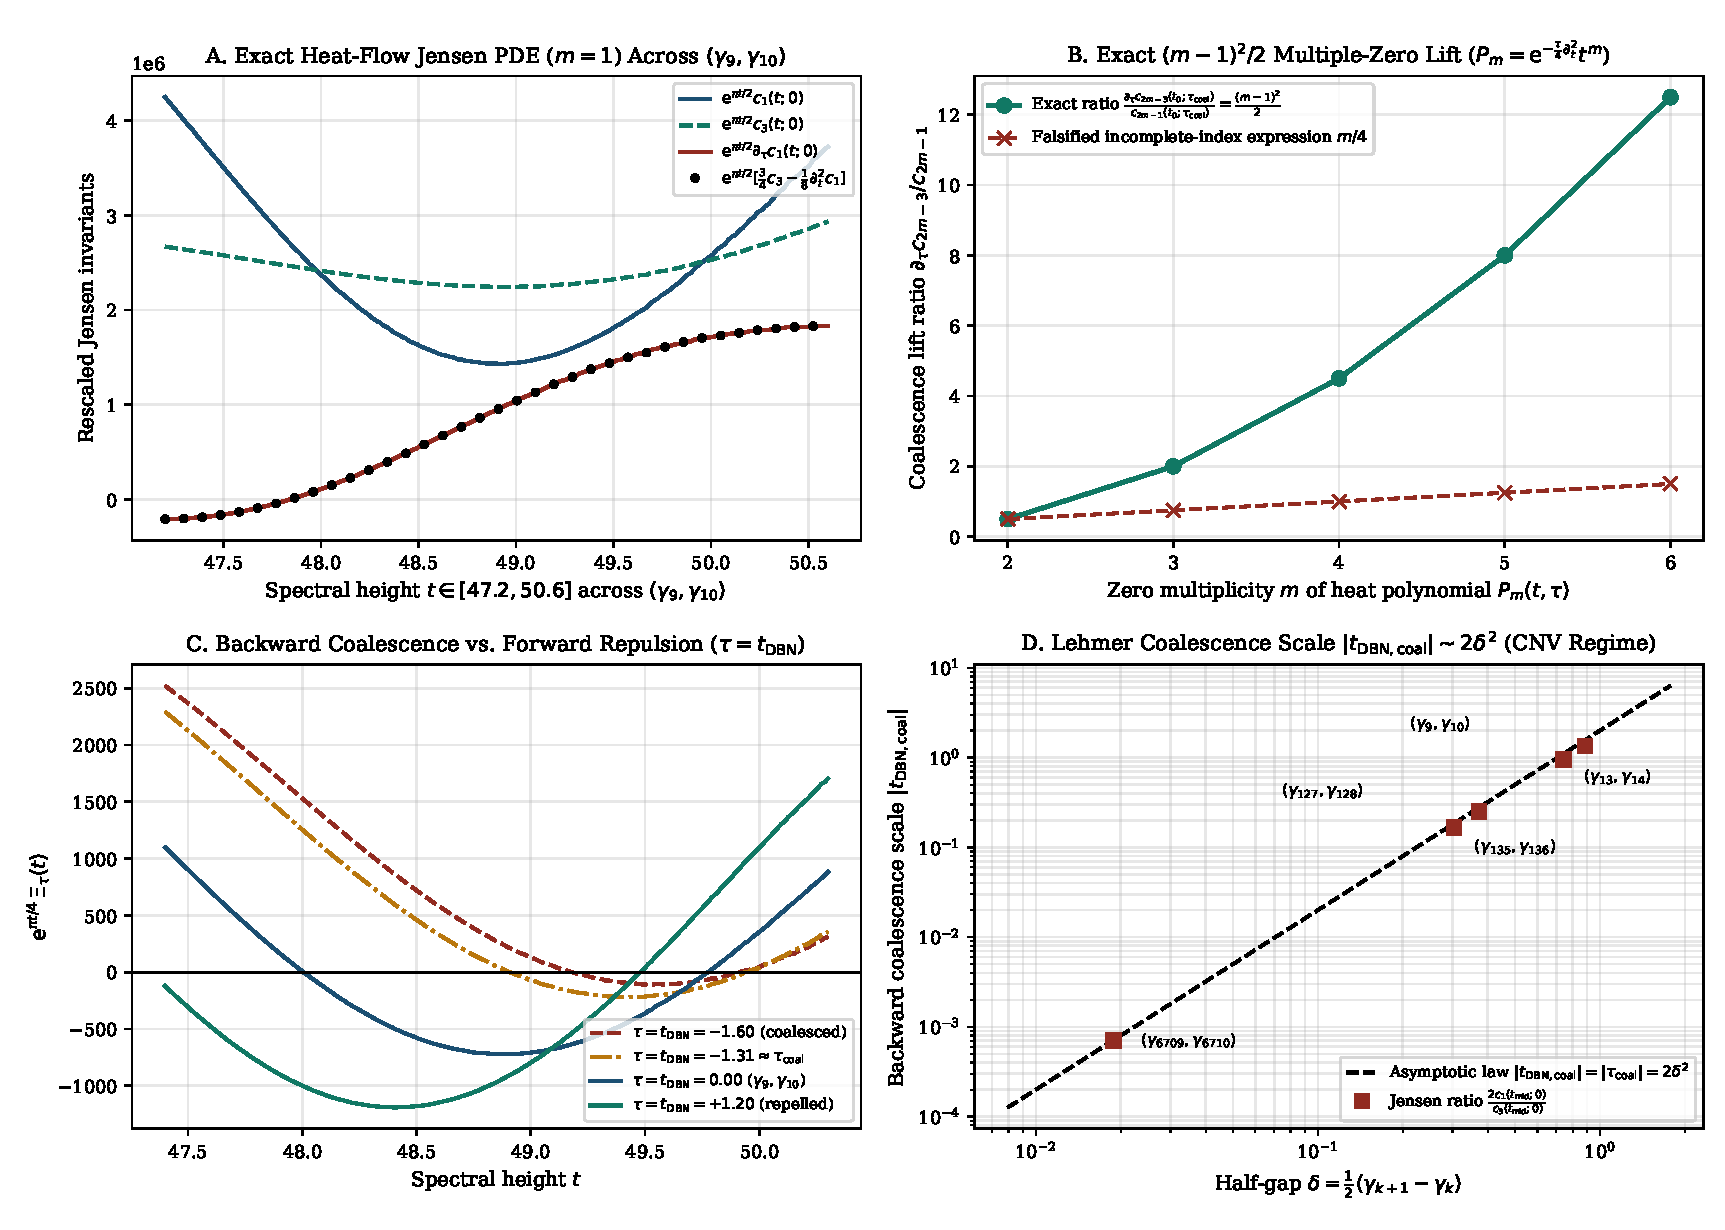
\includegraphics[width=0.97\textwidth]{figures/fig2_dipole_pde_hierarchy_and_lehmer_coalescence.pdf}
\caption{\textbf{A.} Numerical verification of $\partial_\tau c_1 = \frac{3}{4}c_3 - \frac{1}{8}\partial_t^2 c_1$ across $(\gamma_9, \gamma_{10})$. \textbf{B.} Exact multiple-zero lift ratio $\partial_\tau c_{2m-3}/c_{2m-1} = (m-1)^2/2$ on heat polynomials $P_m(t,\tau) = \ee^{-\frac{\tau}{4}\partial_t^2}t^m$ ($m = 2,\dots,6$) versus the incomplete-index expression $m/4$. \textbf{C.} Backward coalescence and forward repulsion of $(\gamma_9, \gamma_{10})$ in $\tau = t_{\mathrm{DBN}}$. \textbf{D.} Log-log scaling of $\lvert t_{\mathrm{DBN,dip}}\rvert \sim 2\delta^2$ across the five pairs of \Cref{tab:lehmer}.}\label{fig:fig2}
\end{figure}

\section{Scope, limitations, and open questions}\label{sec:scope}

We summarize the exact analytical scope and open problems of this manuscript:
\begin{enumerate}[label=\textup{(\arabic*)},leftmargin=2.2em]
\item \textbf{Unconditional differential identities.} With $\tau = t_{\mathrm{DBN}}$ and canonical $W_\tau(d,t) = 16\int_0^\infty y\sinh(2dy)I_\tau(y,t)\dd y$, the nodal-curvature velocity relations~\eqref{eq:zero_velocity_curvature}--\eqref{eq:extremum_velocity_curvature}, the mirror factorization~\eqref{eq:mirror_factor}, the second-order radial wave-heat PDE~\eqref{eq:wave_heat_M_W}, the Jensen--Laguerre heat-flow hierarchy~\eqref{eq:boxed_jensen_pde}, and the $(m-1)^2/2$ multiple-zero coalescence lift~\eqref{eq:exact_mfold_lift} hold unconditionally.
\item \textbf{Domain restrictions, conditional inequalities, and $\Lambda$.} Because $G_{0,\tau}(\ii\eta)$ vanishes at $2\eta_0 = 0.63883\dots < \frac{\pi}{4}$, logarithmic pitchfork perturbation holds locally on zero-free subdomains and requires the unproved numerator inequality~\eqref{eq:numerator_condition} for $\partial_\tau\eta_c < 0$. Similarly, $\partial_\tau c_1(t_{\mathrm{mid}}; 0) > 0$ requires $\Xi(t_{\mathrm{mid}})\Xi^{(4)}(t_{\mathrm{mid}}) > -(\Xi''(t_{\mathrm{mid}}))^2$, and backward Lehmer-pair coalescence probes the Csordas--Norfolk--Varga~\cite{csordas1988} lower-bound regime $\Lambda \ge t_{\mathrm{lb}}$ rather than bounding $\Lambda$ from above; since $\partial_\tau$ evolves as a \emph{backward} heat equation in $+\tau$,~\eqref{eq:boxed_jensen_pde} admits no parabolic maximum principle preserving $L_m \ge 0$ for $\tau < 0$ without independent arithmetic input.
\end{enumerate}

\appendix

\section{Symbolic Polynomial Verification of the Heat-Flow Jensen Hierarchy}\label{app:poly_test}

Consider the backward-heat polynomial family
\[
P_m(t,\tau) := \ee^{-\frac{\tau}{4}\partial_t^2}t^m = \sum_{k=0}^{\lfloor m/2\rfloor} \frac{(-1)^k m\fac}{k\fac(m-2k)\fac}\left(\frac{\tau}{4}\right)^k t^{m-2k},
\]
satisfying $\partial_\tau P_m = -\frac{1}{4}\partial_t^2 P_m$ with an $m$-fold root at $(t,\tau) = (0,0)$. For $m = 3$, $P_3(t,\tau) = t^3 - \frac{3}{2}\tau t$, $P_3' = 3t^2 - \frac{3}{2}\tau$, $P_3'' = 6t$, and $P_3''' = 6$. Substituting these derivatives into~\eqref{eq:Lm_def} yields $c_1 = (P_3')^2 - P_3 P_3''$, $c_3 = \frac{1}{6}[3(P_3'')^2 - 4P_3' P_3''']$, and $c_5 = \frac{1}{12}(P_3''')^2$, which simplify directly to
\begin{equation}\label{eq:P3_explicit}
c_1(t;\tau) = 3t^4 + \frac{9}{4}\tau^2, \qquad c_3(t;\tau) = 6t^2 + 6\tau, \qquad c_5(t;\tau) = 3.
\end{equation}
Evaluating~\eqref{eq:boxed_jensen_pde} on~\eqref{eq:P3_explicit} yields $\partial_\tau c_1 = \frac{9}{2}\tau$ and $\partial_t^2 c_1 = 36t^2$, so for $m = 1$ and $m = 2$:
\begin{align}\label{eq:P3_check_m1}
\left(\frac{\partial}{\partial\tau} + \frac{1}{8}\frac{\partial^2}{\partial t^2}\right)c_1(t;\tau) &= \frac{9}{2}\tau + \frac{9}{2}t^2 = \frac{3}{4}\,c_3(t;\tau), \\
\left(\frac{\partial}{\partial\tau} + \frac{1}{8}\frac{\partial^2}{\partial t^2}\right)c_3(t;\tau) &= 6 + \frac{1}{8}(12) = \frac{15}{2} = \frac{2(5)}{4}\,c_5(t;\tau).\label{eq:P3_check_m2}
\end{align}
At $(t,\tau) = (0,0)$, $\partial_\tau c_3(0;0) / c_5(0;0) = 6 / 3 = 2 = \frac{(3 - 1)^2}{2}$, confirming \Cref{thm:jensen_pde} and \Cref{cor:coalescence_lehmer}(i) explicitly (and refuting $m/4 = 3/4$).

\section*{Use of AI and computational verification}

Portions of the symbolic algebra, polynomial test-case checks, literature cross-checks, and numerical verification scripts in this manuscript were developed and audited with the assistance of Google Gemini. All symbolic identities (\texttt{SymPy} for $m = 0,\dots,6$) and $50$-decimal numerical tables were independently verified via \href{https://github.com/thijsmissiaen/paper11-debruijn-newman-chladni-evolution/blob/main/scripts/verify_paper11_debruijn_newman_chladni.py}{\texttt{scripts/verify\_\allowbreak paper11\_\allowbreak debruijn\_\allowbreak newman\_\allowbreak chladni.py}}.

\begin{thebibliography}{99}

\bibitem{ariasdereyna2003}
J.~Arias de Reyna, \emph{X-ray of Riemann's zeta-function}, preprint (2003), \href{https://arxiv.org/abs/math/0309433}{arXiv:math/0309433}.

\bibitem{cravencsordas1989}
T.~C.~Craven and G.~Csordas, \emph{Jensen polynomials and the Tur\'an and Laguerre inequalities}, Pacific J.\ Math.\ \textbf{136} (1989), no.~2, 241--260.

\bibitem{csordas1986}
G.~Csordas, T.~S.~Norfolk, and R.~S.~Varga, \emph{The Riemann hypothesis and the Tur\'an inequalities}, Trans.\ Amer.\ Math.\ Soc.\ \textbf{296} (1986), no.~2, 521--541.

\bibitem{csordas1988}
G.~Csordas, T.~S.~Norfolk, and R.~S.~Varga, \emph{A lower bound for the de~Bruijn--Newman constant $\Lambda$}, Numer.\ Math.\ \textbf{52} (1988), no.~5, 483--497.

\bibitem{csordas1994}
G.~Csordas, W.~Smith, and R.~S.~Varga, \emph{Lehmer pairs of zeros, the de~Bruijn--Newman constant $\Lambda$, and the Riemann Hypothesis}, Constr.\ Approx.\ \textbf{10} (1994), no.~1, 107--129.

\bibitem{debranges1968}
L.~de~Branges, \emph{Hilbert Spaces of Entire Functions}, Prentice-Hall, Englewood Cliffs, NJ, 1968.

\bibitem{debruijn1950}
N.~G.~de~Bruijn, \emph{The roots of trigonometric integrals}, Duke Math.\ J.\ \textbf{17} (1950), 197--226.

\bibitem{hinkkanen1997}
A.~Hinkkanen, \emph{On functions of bounded type}, Complex Variables Theory Appl.\ \textbf{34} (1997), no.~1--2, 119--139.

\bibitem{hudson1974}
R.~L.~Hudson, \emph{When is the Wigner quasi-probability density non-negative?}, Rep.\ Math.\ Phys.\ \textbf{6} (1974), no.~2, 249--252.

\bibitem{jensen1913}
J.~L.~W.~V.~Jensen, \emph{Recherches sur la th\'eorie des \'equations}, Acta Math.\ \textbf{36} (1913), 181--195.

\bibitem{lagarias1999}
J.~C.~Lagarias, \emph{On a positivity property of the Riemann $\xi$-function}, Acta Arith.\ \textbf{89} (1999), no.~3, 217--234.

\bibitem{lehmer1956}
D.~H.~Lehmer, \emph{Extended computation of the Riemann zeta-function}, Mathematika \textbf{3} (1956), 102--108.

\bibitem{newman1976}
C.~M.~Newman, \emph{Fourier transforms with only real zeros}, Proc.\ Amer.\ Math.\ Soc.\ \textbf{61} (1976), no.~2, 245--251.

\bibitem{polya1926}
G.~P\'olya, \emph{Bemerkung \"uber die Integraldarstellung der Riemannschen $\xi$-Funktion}, Acta Math.\ \textbf{48} (1926), 305--317.

\bibitem{polymath2019}
D.~H.~J.~Polymath, \emph{Effective approximation of heat flow evolution of the Riemann $\xi$-function, and a new upper bound for the de~Bruijn--Newman constant}, Res.\ Math.\ Sci.\ \textbf{6} (2019), no.~3, Paper No.~31, 67~pp.

\bibitem{riemann1859}
B.~Riemann, \emph{Ueber die Anzahl der Primzahlen unter einer gegebenen Gr\"osse}, Monatsber.\ K\"onigl.\ Preuss.\ Akad.\ Wiss.\ Berlin (1859), 671--680.

\bibitem{rodgerstao2020}
B.~Rodgers and T.~Tao, \emph{The de~Bruijn--Newman constant is non-negative}, Forum Math.\ Pi \textbf{8} (2020), e6, 62~pp.

\bibitem{speiser1934}
A.~Speiser, \emph{Geometrisches zur Riemannschen Zetafunktion}, Math.\ Ann.\ \textbf{110} (1934), 514--521.

\bibitem{titchmarsh1986}
E.~C.~Titchmarsh, \emph{The Theory of the Riemann Zeta-Function}, 2nd ed., revised by D.~R.~Heath-Brown, Clarendon Press, Oxford, 1986.

\bibitem{wigner1932}
E.~P.~Wigner, \emph{On the quantum correction for thermodynamic equilibrium}, Phys.\ Rev.\ \textbf{40} (1932), 749--759.

\end{thebibliography}

\end{document}
